\chapter{Introduction}

A fundamental goal of quantum technologies is the ability to manipulate and interact with quantum systems in a way that generates useful information, whether for the purpose of gaining insight into the physics governing such systems or in order to solve complex computational problems, as in the case of quantum information processing \reminder{citations}. Despite the fact that quantum mechanics has been established for around a century, we have only recently begun to harness the unique features found in the quantum domain, spurned by and further proliferating the rapid emergence of highly-controllable quantum technologies. 


\iffalse
In the last few decades, the study of many-particle quantum systems far from equilibrium
has risen to prominence, with exciting developments on both experimental and theoretical physics fronts. With the emergence of quantum simulators, such as ultracold atoms in
optical lattices (Schäfer et al., 2020; Langen et al., 2015) and trapped atomic ions (Blatt
and Roos, 2012), it is possible to experimentally study the coherent dynamics of quantum many-body systems for long times. These developments have stimulated considerable
theoretical research (Eisert et al., 2015; Polkovnikov et al., 2010) including thermalization (or the lack thereof) in generic interacting systems (D’Alessio et al., 2016; Deutsch,
2018; Abanin and Papic, 2017; Abanin et al., 2019), and quantum information propaga- ´
tion (Lewis-Swan et al., 2019; Swingle, 2018).
Since it is impossible to study all potential non-equilibrium behaviors in any single
thesis, we will focus particularly on the adiabatic gauge potential (AGP) (Kolodrubetz
et al., 2017), which is also related to the “fidelity susceptibility", as our lens into the general phenomenon. The AGP is the generator of adiabatic deformations between quantum
eigenstates. It also characterizes the distance between nearby eigenstates (also known as the
Fubini-Study metric (Kolodrubetz et al., 2017; Page, 1987; Kobayashi and Nomizu, 1963;
Provost and Vallee, 1980)). It has deep connections to surprising range of topics, including
quantum state preparation (Torrontegui et al., 2013; Guéry-Odelin et al., 2019), quantum
computing (Hartmann and Lechner, 2019; Takahashi, 2017), efficient heat engines (Vil-
2
lazon et al., 2019), quantum speed limits (Bukov et al., 2019), quantum chaos (Pandey
et al., 2020; Villazon et al., 2020), and quantum computational complexity (Wurtz and
Polkovnikov, 2020; Wurtz et al., 2020).
A partial explanation for why the AGP shows up in so many different contexts could
be the ubiquitous nature of adiabatic processes in physics. For example, adiabatic processes occur in quantum annealing (Santoro and Tosatti, 2006; Santoro and Tosatti, 2008)
in the transport of ultra-cold atoms (Krinner et al., 2014), in many-body state engineering (Bernien et al., 2017), and in quantum thermodynamics (Salamon et al., 2009; Rezek
et al., 2009)). Also, adiabatic-related concepts are useful for model-building in theoretical
physics (e.g. adiabatic continuity in Landau’s Fermi-liquid theory).
\fi


\section{Thesis overview}

The structure of this thesis is as follows: in Ch.~\ref{chap:2_adiabaticity} then in Ch.~\ref{chap:3_Quantum_Optimal_control}. And THEN in Ch.~\ref{chap:4_COLD} followed by Ch.~\ref{chap:5_cd_as_costfunc}. Finally, in Ch.~\ref{chap:6_Applications_fidelity} and Ch.~\ref{chap:7_higher_order_agp}. Then a summary in Ch.~\ref{chap:8_Summary} and future outlook in Ch.~\ref{chap:9_Future_directions}.

\begin{figure}[t!]
    \centering
    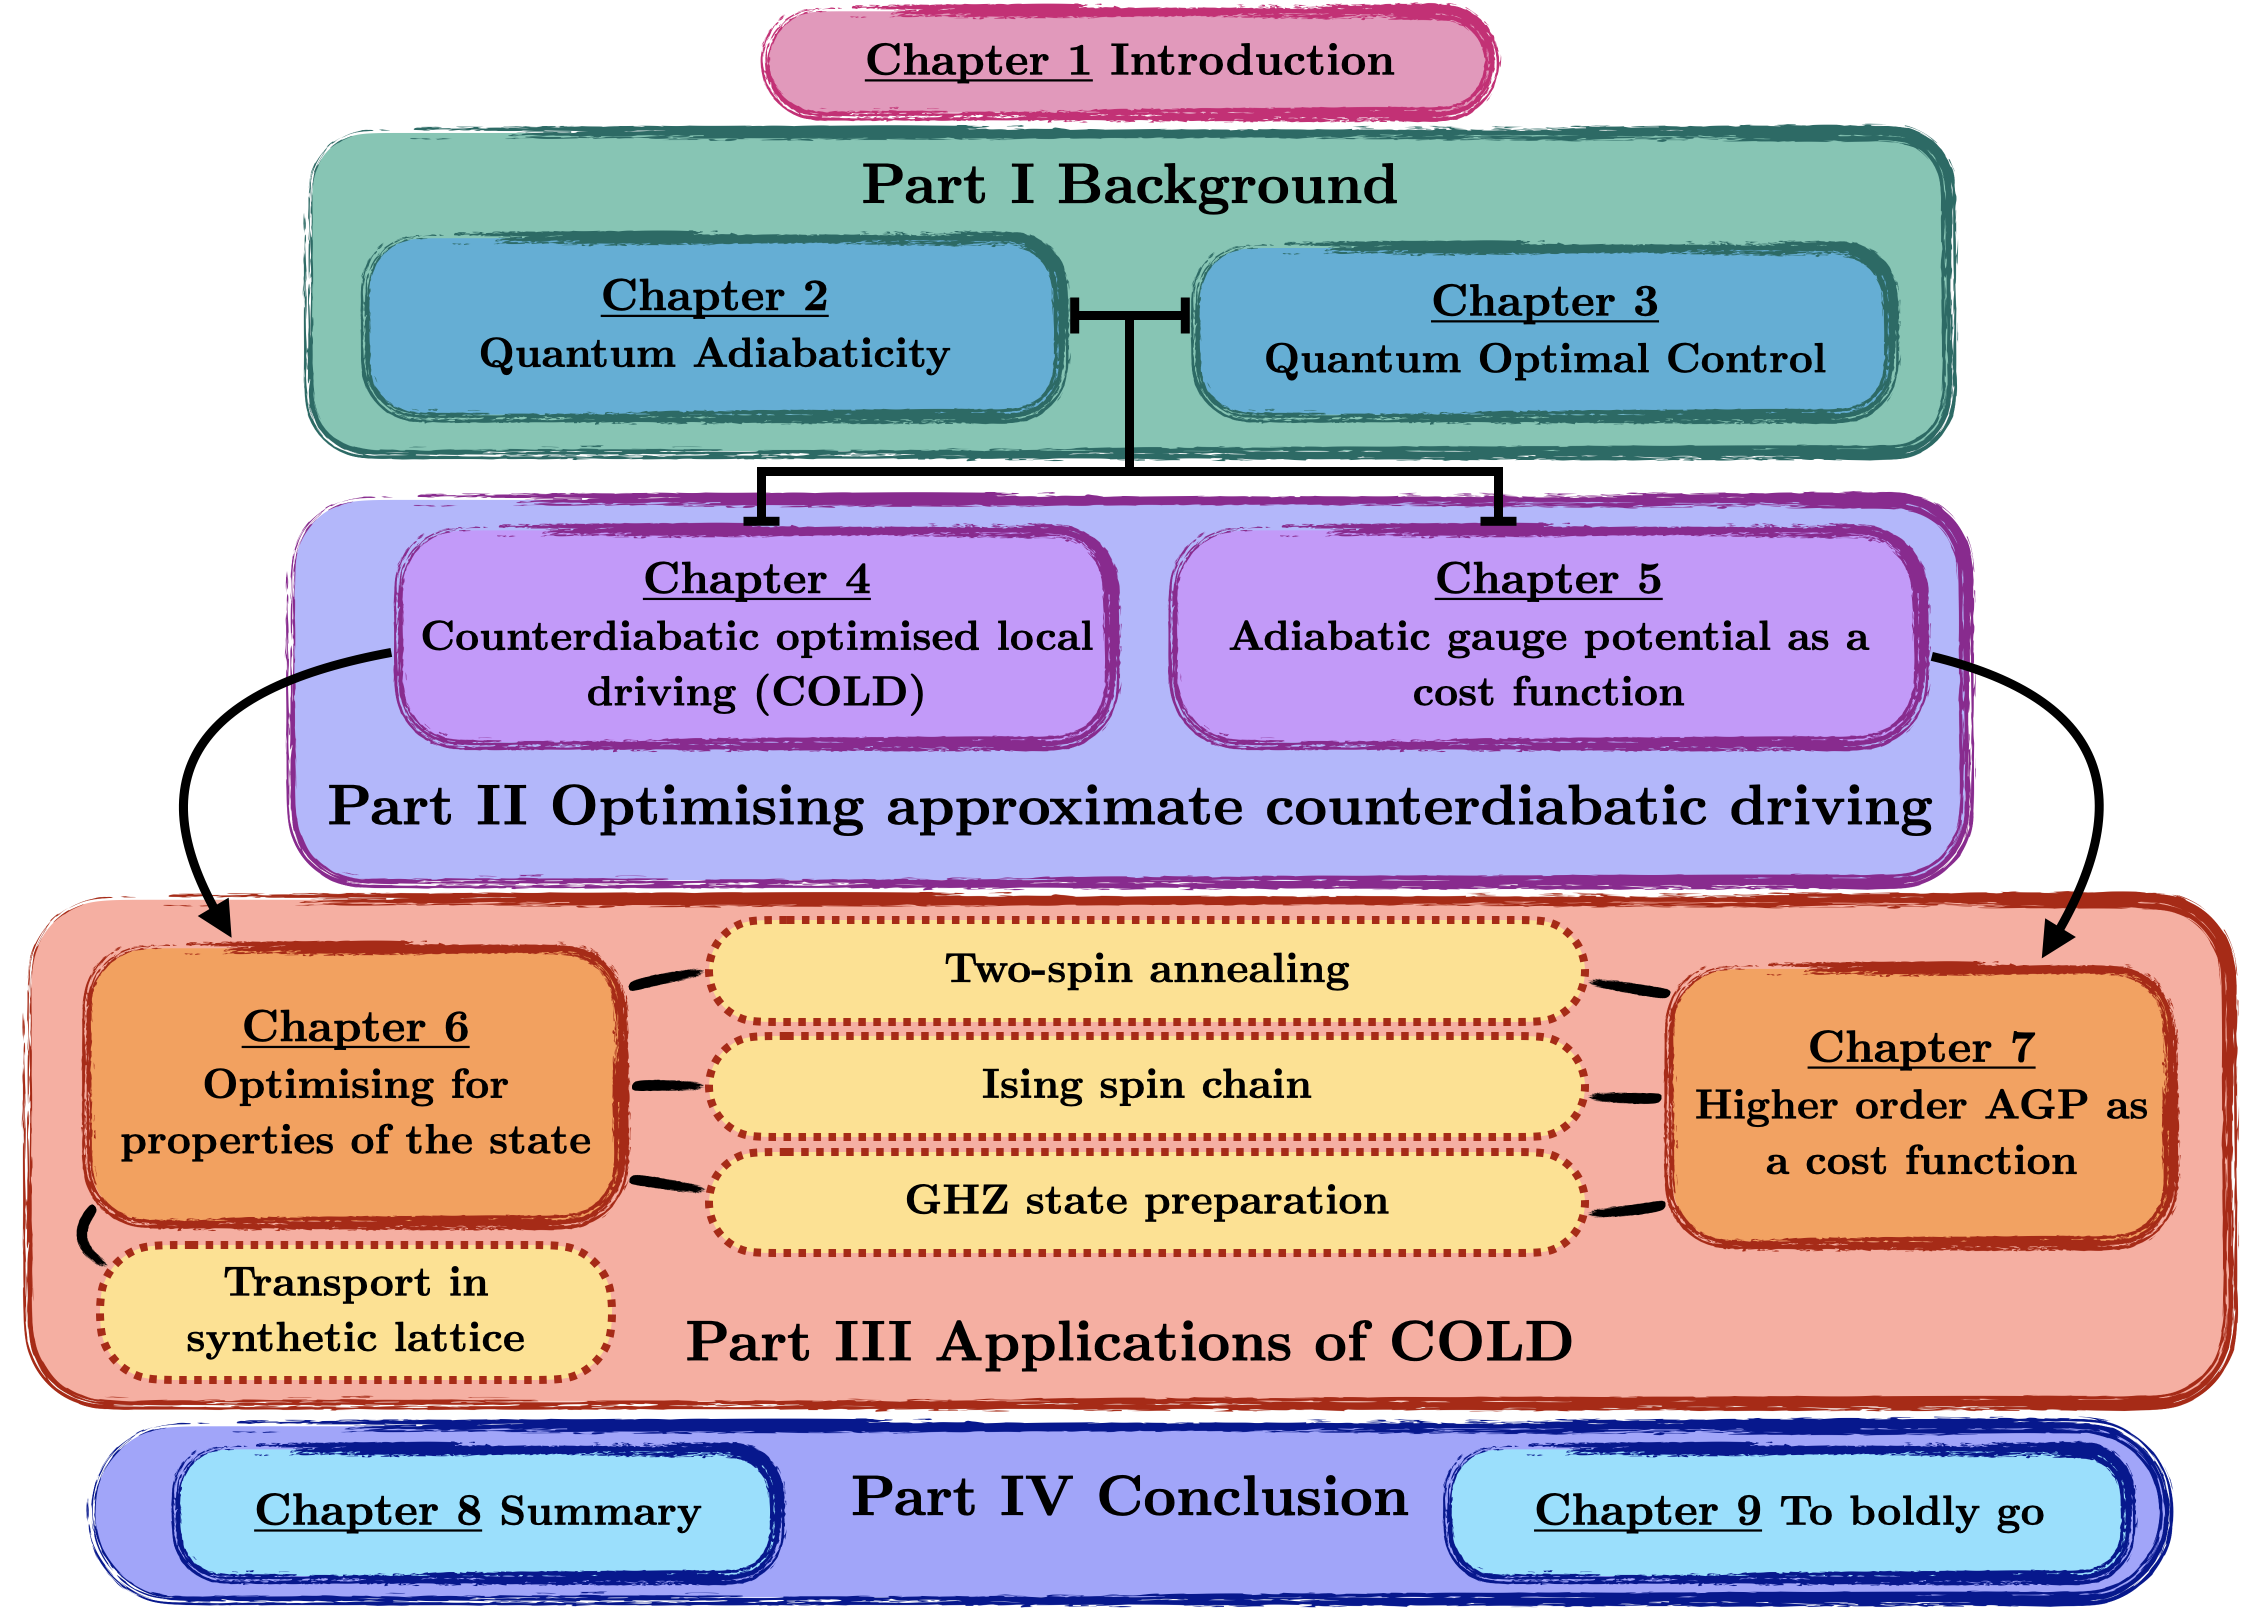
\includegraphics[width=\linewidth]{images/thesis_overview.png} \caption[Thesis outline.]{Thesis outline. In Part~\ref{part:background}, we will introduce the concept of quantum adiabaticity, the counterdiabatic driving (\acrref{CD}) method and its approximations as well as quantum optimal control theory (\acrref{QOCT}) and several optimisation techniques that we will apply later in the thesis. Then, in Part~\ref{part:COLD}, we will combine ideas from \acrref{CD} and \acrref{QOCT} in order to develop a new method for speeding up adiabatic dynamics and the focal point of this thesis: ``Counterdiabatic Optimised Local Driving" or \acrref{COLD}. We will then extend the method with a new optimisation metric based on information about non-adiabatic effects experienced by the system in fast driving. In Part~\ref{part:applications} we will numerically implement the \acrref{COLD} method and its extensions in several different quantum systems to evaluate their performance and compare it to existing techniques. Then, finally, in Part~\ref{part:conclusion}, we will conclude with a summary of the thesis and a look towards the future and several open questions that arise from the work presented here.}\label{fig:thesis_overview}
\end{figure}


\reminder{Here be the context for quantum adiabaticity, include stuff about \acrref{STA} etc.}

\section{Publications and manuscripts}

The majority of this work is based on the following publications and manuscripts:

\begin{enumerate}
    \item \textbf{Counterdiabatic Optimised Local Driving}, \textit{Ieva Čepaitė, Anatoli Polkovnikov, Andrew J. Daley, Callum W. Duncan. PRX Quantum \textbf{4}, 010309, 2023.} Eprint arxiv:2203.01948. \cite{cepaite_counterdiabatic_2023}
    \item \textbf{Many-body spin rotation by adiabatic passage in
    spin-1/2 XXZ chains of ultracold atoms}, \textit{Ivana Dimitrova, Stuart Flannigan, Yoo Kyung Lee, Hanzhen Lin,  Jesse Amato-Grill, Niklas Jepsen, Ieva Čepaitė, Andrew J. Daley, Wolfgang Ketterle. Quantum Sci. Technol. \textbf{8} 035018, 2023} Eprint arxiv:2301.00218.\cite{dimitrova_many-body_2023}.
    \item \textbf{Numerical approaches for non-adiabatic terms in quantum annealing}, \textit{Ewen D. C. Lawrence, Sebastian Schmid, Ieva Čepaitė, Peter Kirton, Callum W. Duncan} Eprint arxiv:0000.00000.
\end{enumerate}

\section{Talks and presentations}

\begin{itemize}
    \item \textit{``Solving Partial Differential Equations (PDEs) with Quantum Computers"}, Atomic Weapons Establishment, (March 2020)
    \item \textit{``A Continuous Variable Born Machine"}, \href{https://www.youtube.com/live/ImQeEs0BcQs?feature=share&t=1996}{Pittsburgh Quantum Institute Virtual Poster Session}, Online (April 2020)
    \item \textit{``A Continuous Variable Born Machine"}, \href{https://www.youtube.com/watch?v=6v1IiXRToPU&t=3685s}{Quantum Techniques in Machine Learning}, Online (November 2020)
    \item \textit{``Variational Counterdiabatic Driving"}, University of Strathclyde and University of Waterloo Joint Virtual Research Colloquium on Quantum Technologies, Online (November 2020)
    \item \textit{``A Continuous Variable Born Machine"}, Bristol QIT Online Seminar Series, Online (March 2021)
    \item \textit{``Optimised counderdiabatic driving with additional terms"}, \href{https://meetings.aps.org/Meeting/MAR21/Session/S21.8}{APS March Meeting}, Online (March 2021)
    \item \textit{``Counterdiabatic Optimised Local Driving"}, \href{https://www.youtube.com/watch?v=YkoCPIlFl70}{DAMOP}, Orlando (May 2022)
    \item \textit{``Counterdiabatic Optimised Local Driving"}, QCS Hub Project Forum, Oxford (January 2023)
    \item \textit{``Counterdiabatic Optimised Local Driving"}, \href{https://meetings.aps.org/Meeting/MAR23/Session/Q71.8}{APS March Meeting}, Las Vegas (March 2023)
    \item \textit{``Counterdiabatic Optimised Local Driving"}, \href{https://youtu.be/-btmXDNaQX4}{INQA Seminar}, Online (March 2023)
\end{itemize}